\section{Implementation Plan}
The implementation of Data4Help and AutomatedSOS systems is carried on taking into consideration some important factors, such as the complexity of each component and its relations with the other ones. Of course, the implementation plan takes into special consideration the core components which are essential for the whole system and are considered as \say{bottleneck}. 
It is important to fix any flaws as soon as it is detected, so that the correction costs in terms of time are kept the lower possible.
The order in which our system is implemented is the following:

\begin{enumerate}
    \item Model
    \item Central Controller
    \item Account Manager
    \item Third party services, User Services
    \item Emergency Service
    \item Web, Mobile and Wearable Applications
\end{enumerate}
\begin{figure}[H]
    \makebox[\textwidth]{
        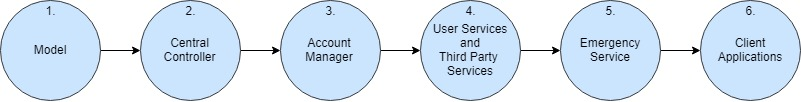
\includegraphics[width=1.3\linewidth]{images/Integration_plan.jpg}
    }
\end{figure}

\subsubsection{Model}
The Model is the first step of the implementation plan, according to its vital role for the whole application.
Since the classes of the Model are used by all the components, it is important that they are ready as soon as possible and are used as a reference. Otherwise each team member would implement the classes of the Model \say{on the fly} when he/she needs them, introducing possible implementation flaws or not using abstraction in a proper way.

\subsubsection{Central Controller}
This component is the logic core of the application. According to this, it requires lot of time to be implemented and, consequently, it is a risky component. It is important that the least possible flaws are inserted during its implementation, since it may have catastrophic consequences in terms of time costs. An important non functional requirement is the fault tolerance and the high throughput. This component may is stressed with lots of requests by each user and third party and it has to react in a short while. For this reason, this component is consider as a \say{bottleneck}.

\subsubsection{Account Manager}
This module allows the sign-up and login of the users and third parties and also is used by the Central Controller when a third party compose a request for data of a specific user. As shown in the \hyperlink{RV}{\underline{Runtime view, section 2.5}}, the third party fills the request form specifying the user's SSN or Fiscal Code and, thanks to the Account Manager, the Central Controller converts it into the corresponding user ID.
This module is used for the login and sign-up processes by both users and third parties and, consequently, it has to use abstraction to achieve this interdependence.

\subsubsection{Third party services, User Services}
This two components allow the interaction between the user application(mobile or wearable) and the third party application(mobile or web), passing through the Central Controller.
They can be implemented together since they are quit similar to each other.
As shown in the \hyperlink{CV}{\underline{Component view, section 2.5}}, the sub-components that allows the login, the registration and the access to data are the same in the two module. 
Regarding to the Individual and the group requests, the Third party services component offers the possibility to create them while the User services component allow the user to manage them.
According to what just said, they are implemented just after the Central Controller and the Account Manager.

\subsubsection{Emergency Service}
This component has a vital role for the AutomatedSOS system. It analysis real-time health parameters by comparing them with specific thresholds. It has a strictly dependence with the User services component and with the Central Controller, so that it has to be implemented just after they are ready to use.
Of course, Emergency Service has to be fault tolerant since it deals with human lives. In this component, in the case that a fault appears, it has to be recovery as soon as possible since the system must result available 24/7. 
This component must guarantee an high throughput since it receives a large amount of real-time health data from all the users at the same time.

\subsubsection{Web, Mobile and Wearable Applications}
The last part of the system that has to be implemented consists on the applications. They allow user and third party to interacts with the system, so that they don't have a core function for the system.
They represent only a minimum part of the code and they require short while to be implemented. 
Their implementation will be independent from the Operative System of the device on which they will run.
The application must properly run on different devices concerning the users(smart-phones and wearable-devices) and concerning the third parties(personal computers, tablets and smart-phones). 
For these reasons, application components are not considered \say{risky} and they are taking into consideration as the last part of the implementation plan.

\clearpage
\section{Integration and Testing}
 \subsection{Entry Criteria}
\subsection{Elements to be Integrated}
\subsection{Integration Testing Strategy}
\subsection{Sequence of Component/Function Integration}